\subsubsection{Use case diagram}
	A global picture of the system interaction with actors is provided here by means of use case diagrams. Following, an analysis of the most interesting use case situations derived from scenarios is presented.

	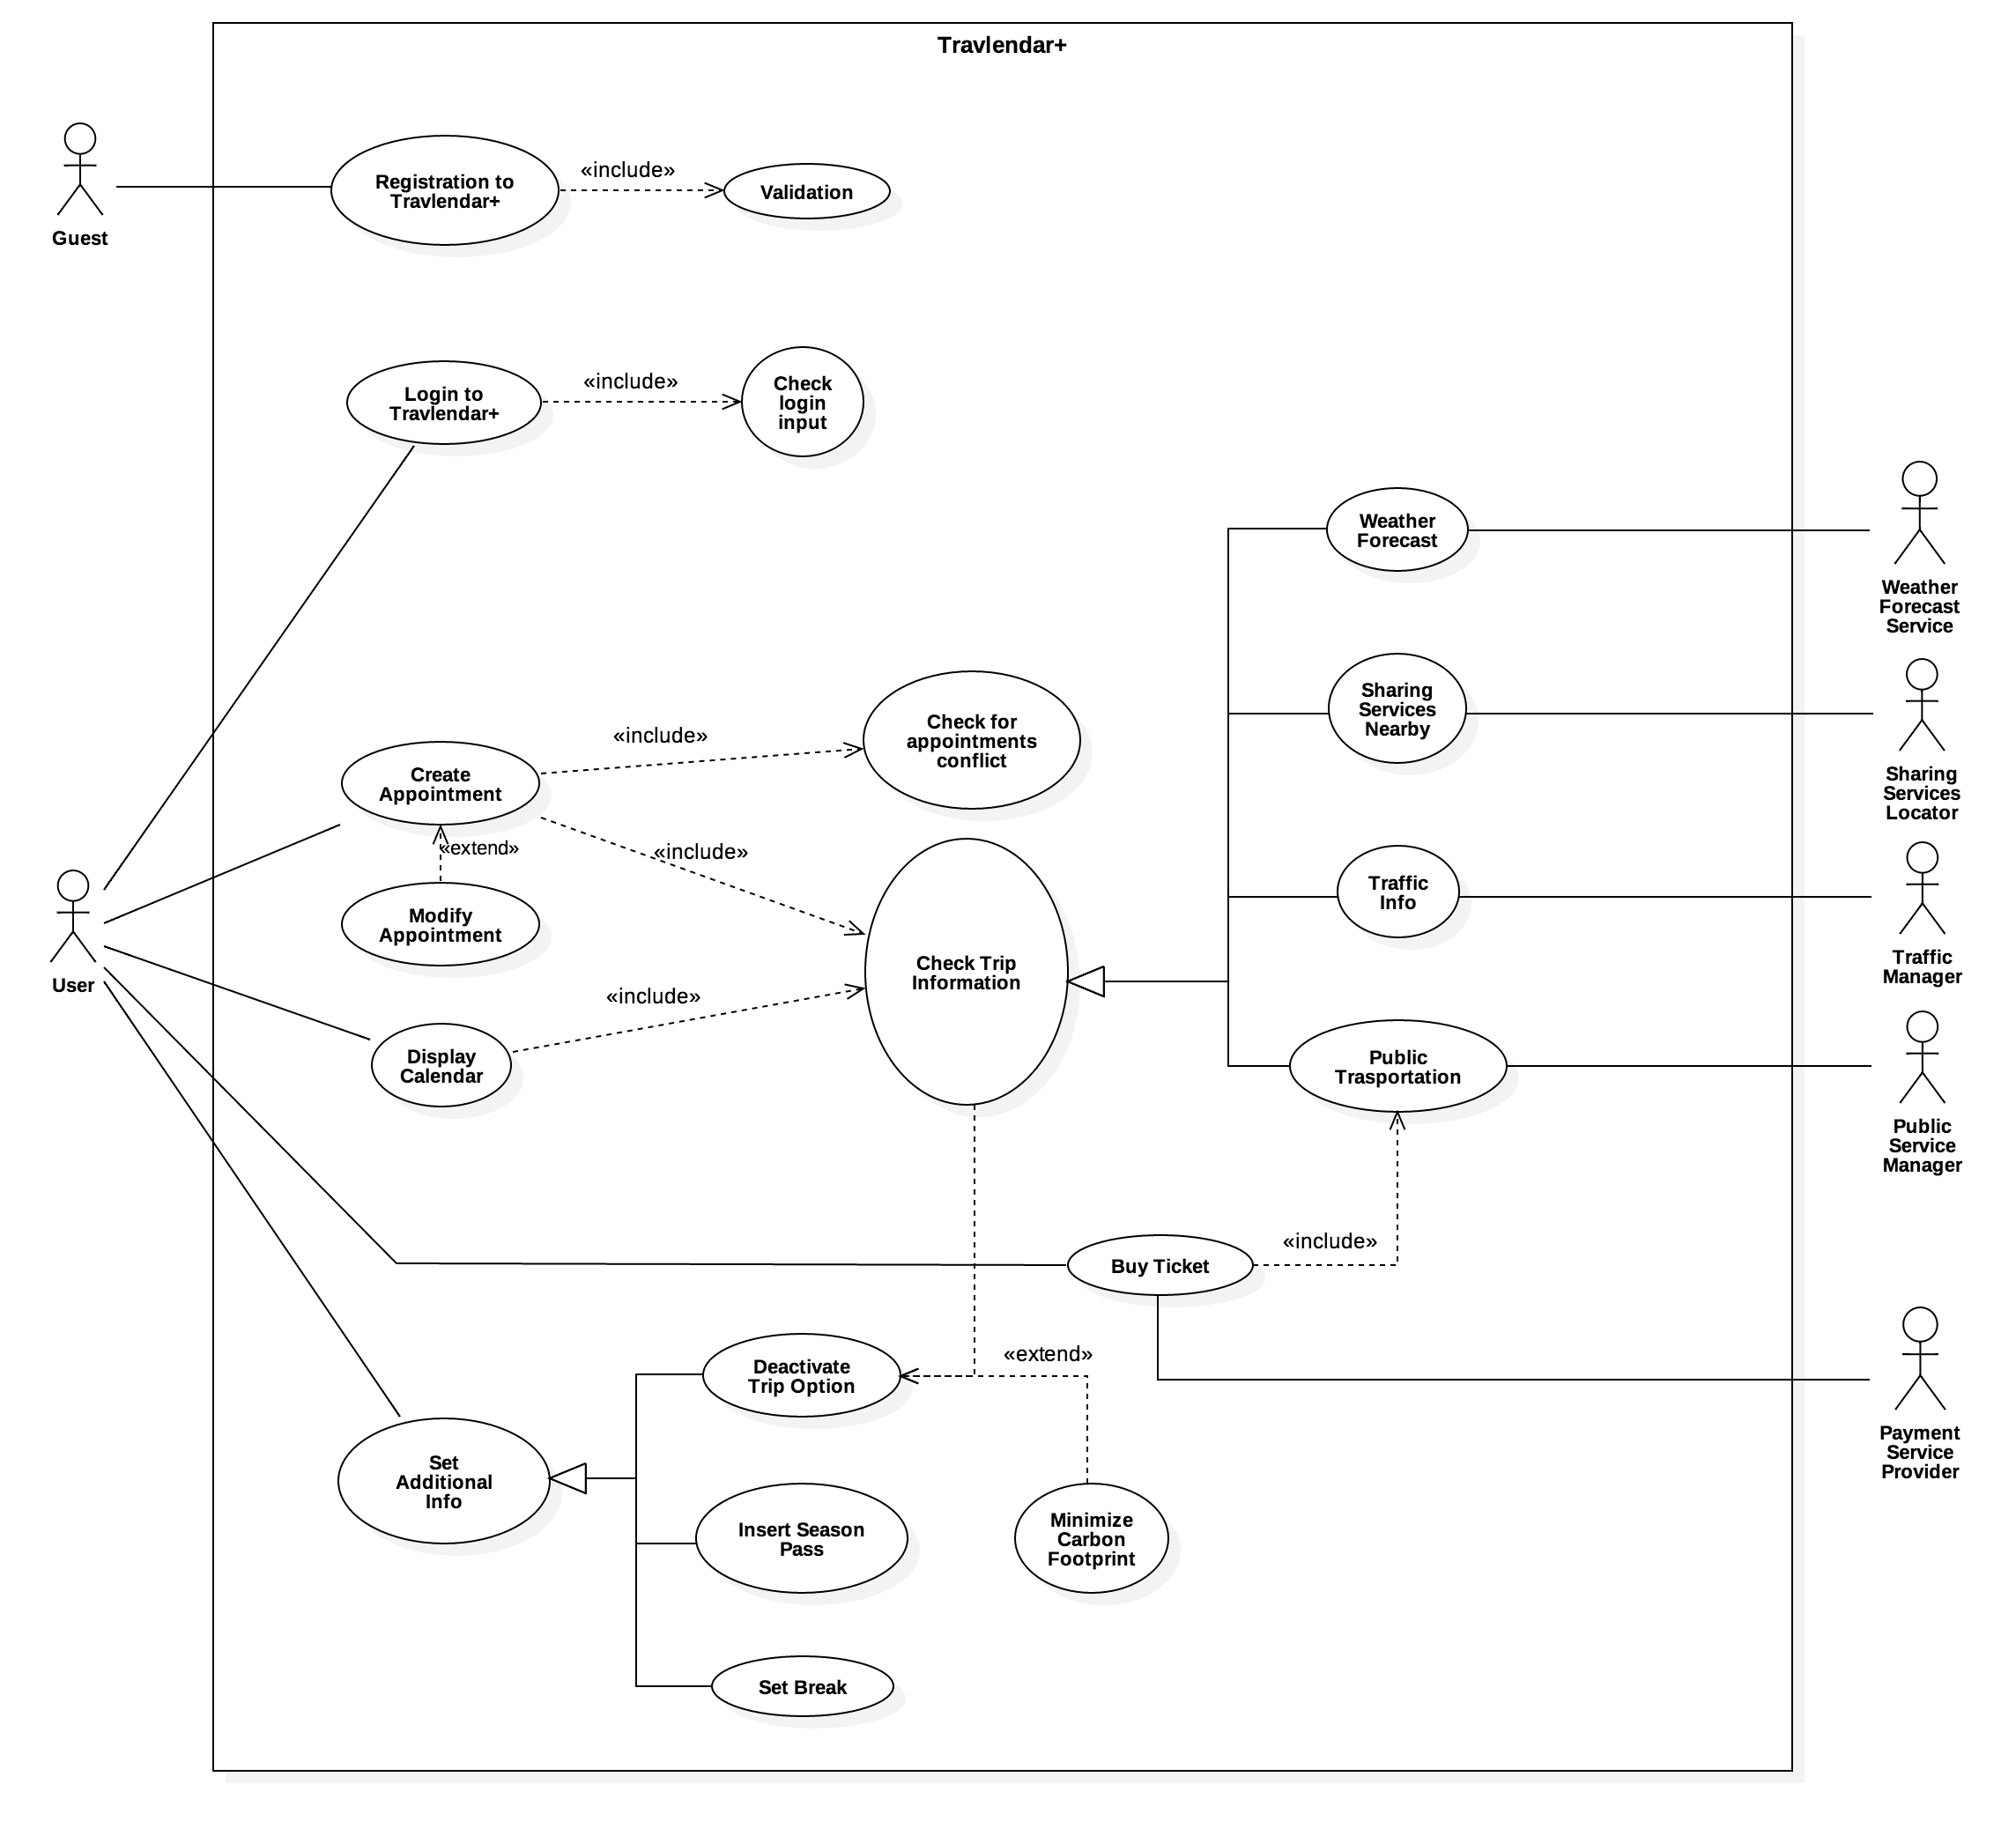
\includegraphics[width=\textwidth]{img/uml/useCase.png}

%%% CREATE A NEW EVENT %%%	
	\paragraph{Use Case 1: Create a New Event}
	
		\begin{tabular}{| l | p{0.8\textwidth} | }
			\hline
			\hline
			Actor	&		User. \\
			\hline
			Input Condition		&		User is already logged in into \textit{Travlendar+}. \\
			\hline
			Event Flow		&		\begin{enumerate}
												\item User click on "\textit{create event}".
												\item User set day, time, place, and event type.
												\item System checks if the new event overlap with already existing events or lunch period.
												\item	 System calculate, ranks and shows multiple solution depending on user travelling preferences.
												\item User select one solution as preferend one.
											\end{enumerate} \\
			\hline
			Output Condition		&		\textit{Tralvendar+} shows calendar main page with the new event. \\
			\hline		
			Exception		&		\begin{itemize}
											\item[-] Created event overlaps with already existing events.
											\item[-] There are no feasible solution.
										\end{itemize} \\
			\hline
			\hline
		\end{tabular}


%%% MODIFY EVENT %%%

	\paragraph{Use Case 2: Modify Event}
	
		\begin{tabular}{| l | p{0.8\textwidth} | }
			\hline
			\hline
			Actor	&		User. \\
			\hline
			Input Condition		&		\begin{itemize}
													\item[-] User is already logged in into \textit{Travlendar+}.
													\item[-] Event Already Exists.
												\end{itemize} \\
			\hline
			Event Flow		&		\begin{enumerate}
												\item User click on "\textit{Event}".
												\item User starts modifying process.
												\item System checks if the new event overlap with already existing events or lunch period.
												\item	 System calculate, ranks and shows multiple solution depending on user travelling preferences.
												\item User select one solution as preferend one.
											\end{enumerate} \\
			\hline
			Output Condition		&		\textit{Tralvendar+} shows calendar main page, with the updated event. \\
			\hline		
			Exception		&		\begin{itemize}
											\item[-] Created event overlaps with already existing events.
											\item[-] There are no feasible solution.
										\end{itemize} \\
			\hline
			\hline
		\end{tabular}
		
		
%%% INSERT PAYMENT METHOD%%%

	\paragraph{Use Case 3: Insert Payment Method}
	
		\begin{tabular}{| l | p{0.8\textwidth} | }
			\hline
			\hline
			Actor	&		User. \\
			\hline
			Input Condition		&		\begin{itemize}
													\item[-] User is already logged in into \textit{Travlendar+}.
													\item[-] Credit Card isn't already inserted on the system.
												\end{itemize} \\
			\hline
			Event Flow		&		\begin{enumerate}
												\item User click on "\textit{Preferences}" and then on "\textit{Payment Methods}".
												\item User sets all the credit cards info.
												\item System checks and validate provided informations.
											\end{enumerate} \\
			\hline
			Output Condition		&		\textit{Tralvendar+} returns to \textit{Payment Methods} page showing added card as a valid payment method. \\
			\hline		
			Exception		&		Credit card given informations are invalid. \\
			\hline
			\hline
		\end{tabular}

%%% BUY TICKET %%%

	\paragraph{Use Case 4: Buy Public Transportation Ticket}
	
		\begin{tabular}{| l | p{0.8\textwidth} | }
			\hline
			\hline
			Actor	&		User. \\
			\hline
			Input Condition		&		\begin{itemize}
													\item[-] User is already logged in into \textit{Travlendar+}.
													\item[-] A \textit{payment method} is already available.
												\end{itemize} \\
			\hline
			Event Flow		&		\begin{enumerate}
												\item User click on "\textit{Buy Ticket}".
												\item System shows available public trasportation services.
												\item User selects a ticket.
												\item	 System starts perchause transaction.
											\end{enumerate} \\
			\hline
			Output Condition		&		Based on public transportation service, User receives a valid ticket. \\
			\hline		
			Exception		&		Transaction doesn't work. \\
			\hline
			\hline
		\end{tabular}
